% Figure 5.2: Data Flow Diagram
% Compile with: pdflatex fig_5_2_data_flow.tex

\documentclass[border=10pt]{standalone}
\usepackage{tikz}
\usetikzlibrary{shapes.geometric, arrows.meta, positioning}
\usepackage{xcolor}

% Professional academic color palette
\definecolor{layer1}{RGB}{70, 130, 180}        % Steel blue
\definecolor{layer2}{RGB}{100, 149, 237}       % Cornflower blue
\definecolor{layer3}{RGB}{119, 136, 153}       % Light slate gray
\definecolor{accentteal}{RGB}{119, 176, 166}   % Muted teal
\definecolor{databg}{RGB}{240, 240, 240}       % Light gray
\definecolor{textdark}{RGB}{33, 33, 33}

\begin{document}
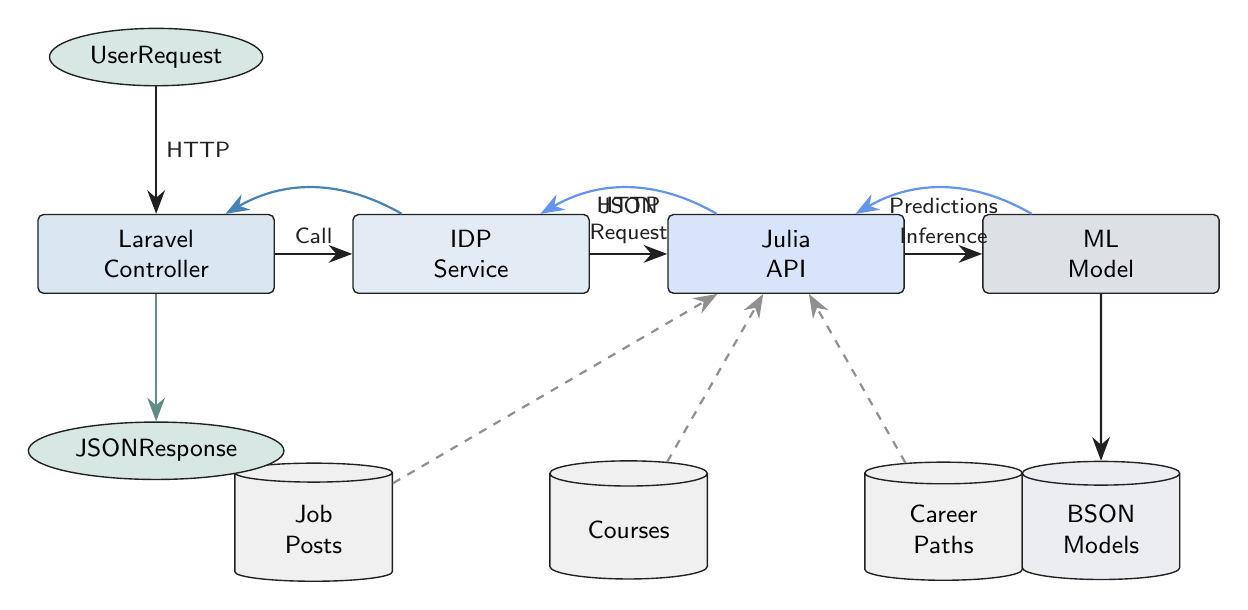
\begin{tikzpicture}[
    node distance=2cm,
    process/.style={rectangle, draw=textdark, rounded corners=2pt, fill=layer2!25, minimum width=3cm, minimum height=1cm, align=center, font=\small\sffamily, line width=0.5pt},
    data/.style={cylinder, draw=textdark, fill=databg, shape border rotate=90, aspect=0.25, minimum height=1.5cm, minimum width=2cm, align=center, font=\small\sffamily, line width=0.5pt},
    arrow/.style={-{Stealth[length=3mm]}, thick, color=textdark},
    label/.style={font=\footnotesize\sffamily, align=center, color=textdark}
]

% User Request
\node[ellipse, draw=textdark, fill=accentteal!30, minimum width=2.5cm, font=\small\sffamily, line width=0.5pt] (user) at (-6, 4) {User\\Request};

% Laravel
\node[process, fill=layer1!20] (laravel) at (-6, 1.5) {Laravel\\Controller};

% Service
\node[process, fill=layer1!15] (service) at (-2, 1.5) {IDP\\Service};

% API
\node[process, fill=layer2!25] (api) at (2, 1.5) {Julia\\API};

% Models
\node[process, fill=layer3!25] (model) at (6, 1.5) {ML\\Model};

% Data sources
\node[data] (jobdata) at (-4, -2) {Job\\Posts};
\node[data] (coursedata) at (0, -2) {Courses};
\node[data] (careerdata) at (4, -2) {Career\\Paths};

% Model files
\node[data, fill=layer3!15] (bson) at (6, -2) {BSON\\Models};

% Response
\node[ellipse, draw=textdark, fill=accentteal!30, minimum width=2.5cm, font=\small\sffamily, line width=0.5pt] (response) at (-6, -1) {JSON\\Response};

% Arrows
\draw[arrow] (user) -- node[right, label] {HTTP} (laravel);
\draw[arrow] (laravel) -- node[above, label] {Call} (service);
\draw[arrow] (service) -- node[above, label] {HTTP\\Request} (api);
\draw[arrow] (api) -- node[above, label] {Inference} (model);
\draw[arrow] (model) -- (bson);
\draw[arrow, dashed, color=textdark!50] (jobdata) -- (api);
\draw[arrow, dashed, color=textdark!50] (coursedata) -- (api);
\draw[arrow, dashed, color=textdark!50] (careerdata) -- (api);

% Return path
\draw[arrow, color=layer2] (model) to[bend right=30] node[below, label] {Predictions} (api);
\draw[arrow, color=layer2] (api) to[bend right=30] node[below, label] {JSON} (service);
\draw[arrow, color=layer1] (service) to[bend right=30] (laravel);
\draw[arrow, color=accentteal!80!black] (laravel) -- (response);

\end{tikzpicture}
\end{document}
